\documentclass[3p, a4paper, authoryear, 11pt, fleqn, review]{elsarticle}
\usepackage{acronym}
\usepackage[linesnumbered, ruled, vlined]{algorithm2e}
\usepackage{amsmath,amssymb,amsfonts}
\usepackage{siunitx}
\usepackage{graphicx}
\graphicspath{
	{./graphics/}
}
\usepackage{hyperref}

\usepackage[left,mathlines]{lineno}
\usepackage{enumitem}
\usepackage[normalem]{ulem}
\usepackage{pdflscape}


\usepackage{natbib}
	\bibliographystyle{apalike}

\hypersetup{
  	bookmarks=true,         % show bookmarks bar?
    unicode=false,          % non-Latin characters in Acrobat's bookmarks
    pdftoolbar=true,        % show Acrobat's toolbar?
    pdfmenubar=true,        % show Acrobat's menu?
    pdffitwindow=true,      % page fit to window when opened
    pdftitle={}, 	% title
    pdfauthor={},   % author
    pdfsubject={},% subject of the document
    pdfnewwindow=true,      % links in new window
    pdfkeywords={},			%list of keywords
    colorlinks=true,   		% false: boxed links; true: colored links
    linkcolor=blue,        	% color of internal links
    citecolor=blue, 		% color of links to bibliography
    filecolor=blue,      	% color of file links
    urlcolor=blue           % color of external links
}	
\usepackage{subfig}
\usepackage{soul}
\usepackage{float}
\usepackage{supertabular}
\usepackage{booktabs}
\usepackage{textcomp}
\usepackage{multirow}
\usepackage{multicol}
\usepackage{array}
\newcolumntype{L}[1]{>{\raggedright\let\newline\\\arraybackslash\hspace{0pt}}m{#1}}
\newcolumntype{C}[1]{>{\centering\let\newline\\\arraybackslash\hspace{0pt}}m{#1}}
\newcolumntype{R}[1]{>{\raggedleft\let\newline\\\arraybackslash\hspace{0pt}}m{#1}}
\usepackage{url}
\usepackage{booktabs}

%This clashes with pdfpages package
\usepackage[dvipsnames]{xcolor}
\newcommand{\nmt}[1]{{\color{ForestGreen}{~(nmt: #1)}}}

\usepackage{pdfpages}



\title{Logistics sprawl in New Zealand's urban centres between 2000--2020}

%\author{\textbf{Anonymous, for review}}

\author[UW]{Nadia M. Trent\fnref{ead1}}
\fntext[ead1]{ nadia.trent@waikato.ac.nz (N.M. Trent, corresponding author)}


%\author[UP1]{Johan W. Joubert\fnref{ead2}}
%\fntext[ead2]{ johan.jouberth@up.ac.za (J.W. Joubert)}



\address[UW]{School of Management and Marketing, University of Waikato}
%\address[UP1]{Department of Industrial and Systems Engineering, University of Pretoria}



\journal{(early draft)}

\begin{document}
\acrodef{OSM}{OpenStreetMap}
\acrodef{NZDep}{New Zealand Deprivation}
\acrodef{ANZSIC}{Australia and New Zealand Standard Industrial Classification}
\acrodef{SA2}{Statistical Area 2}
\acrodef{RET}{Retail}
\acrodef{WSL}{Wholesale}
\acrodef{TWD}{Transport, warehouse \& distribution}
\acrodef{StatsNZ}{Statistics New Zealand}
\acrodef{CAGR}{compound annual growth rate}
\acrodef{GTWR}{geographically and temporally weighted regression}




\begin{abstract}\small
Some abstract
\end{abstract}

\begin{keyword}
keyword 1
\end{keyword}


\maketitle


\section{Introduction}
\label{sec:Intro}

\nmt{NADIA: Is city logistics really the right term to use here? I don't see a firm home for logistics sprawl research under the city logistics umbrella}
\nmt{Common ground} Between 2000 and 2021, the population of Aotearoa New Zealand grew by 33\% from just over 3.8\,million people to just over 5.1\,million people. The average annual growth rate between 2000 and 2013 was 1.06\% per year. This average rose to 1.96\% between 2014 and 2020. The 2021 estimate of annual growth, which reflects the impact of a full year of border closures, has dropped to 0.64\% \nmt{ref StatsNZ} and is the first time since 2013 that natural increase (births minus deaths) drove population growth \nmt{https://www.stats.govt.nz/news/births-drive-population-growth}.  

While the role of international immigration in Aotearoa New Zealand's robust population growth is a central topic in policy discourse \nmt{Book chapter}, it is not the only one. Concerns regarding the ageing population and asymmetrical regional growth also feature prominently and hold strong social and economic implications \nmt{Michael Cameron?, Brabyn and Jackson}. \nmt{Complication} But the discourse on population growth and, specifically, the growth of urban areas, is missing a key perspective: that of the urban freight systems (also called city logistics) which develop alongside expanding industries and bulging consumer bases.

\nmt{This needs more careful thought} City logistics is a broad term that encompasses \nmt{...}. Over the past decade, many scholars have pursued an understanding of city logistics by studying, among other phenomena: logistics sprawl, clustering\nmt{?}, and distention \nmt{refs}; freight landscapes \nmt{extend phrase and add}; and \nmt{holguin veras work...  and other elements of city logistics}. The motivating thrust for this work has been the impact that city logistics have on the economy, society, and the environment \nmt{Aljohani Thompson and others.}.

\nmt{Expand on impact and why it's important}

\nmt{Concern} Studies conducted in cities across the world underscore the influence of the local context --- such as a city's urban form, demographics, and land use policies --- on the city logistics that emerge in that place. Therefore, while these global studies about city logistics highlight issues to explore and offer methodologies to do so, the findings from other cities and countries cannot be taken and applied as-is in Aotearoa New Zealand. \nmt{Course of action} Instead, we need to develop our own understanding of city logistics in our major urban areas. Without such an understanding, policy making could, at best, miss out on opportunities to increase the efficiency of city logistics and, at worst, make decisions that inadvertently worsen the social and environmental impact of city logistics. 


\nmt{Contribution} This paper presents a basis for an ongoing study of city logistics in Aotearoa New Zealand by answering the following research question:
\begin{quote}
\emph{``How has the spatial organisation of urban logistics changed between 2000 and 2020 as a whole and, more specifically, as it intersects with general business and society?''}  	
\end{quote}

We focus the research on the six regions that contain the largest cities in Aotearoa New Zealand: Auckland, Canterbury, Wellington, Waikato, Otago, and Bay of Plenty. Our methodology stems from similar logistics sprawl studies from around the world. 

In the next section we briefly review the body of research on logistics sprawl, highlighting the methodologies relevant to our study \nmt{revise}. In Section~\ref{sec:Method} we describe our data sources and methodologies in detail. The findings of the six regions are presented in Section~\ref{sec:Findings} while Section~\ref{sec:DiscConc} discusses the implications of the findings and concludes by identifying areas of future work. 

\section{Literature review}
\label{sec:LitReview}

\subsection{Logistics sprawl studies}
Urban logistics systems exist because businesses produce goods and services that need to reach other businesses and, ultimately, consumers. Urban logistics is not an end unto itself, it is what emerges from the way we do business, build infrastructure, and manage freight movement in our cities. In terms of doing business: evolving consumer behaviour, supply chain globalisation, and growing populations constantly change the demands placed on urban logistics systems. Meanwhile, prescriptive land use planning, infrastructure development, and regulation and policy impact how urban logistics can respond to that demand. 

\nmt{See if these references still make sense\citep{AljohaniThompson2016, Andreoli_etal2010, He_etal2018, Sakai_etal2015, Kang2020}.}

One of the key phenomena studied around the world as urban logistics systems adapt, is a change in the spatial organisation of logistics facilities in urban areas. Predominantly, studies show that these facilities have become larger and have moved outward from densely populated city centres. This spatial deconcentration is termed ``logistics sprawl" \citep{Dablanc 2014} and has been observed in Europe \citep{DablancRakotonarivo2010, Heitz_etal2020, Kumhalova2019,Strale2020}, North America \citep{Cidell2010, Jaller_etal2017, Kang2020, Kang2020b, Kang2020c}, Asia \citep{He_etal2019, LimPark2020, Sakai_etal2015, Sakai_etal2017}, India \citep{GuptaGarima2017}, and South Africa \nmt{our paper} \nmt{might want to add some refs or reshuffle so as not to be exact copy and paste}. However, logistics sprawl is not a given in growing urban areas as the examples of Seattle \citep{Dablanc_etal2014}, the Noord Holland and Zuid Holland provinces in the Netherlands \citep{Heitz_etal2017}, S\~ao Paulo Metropolitan Region in Brazil \nmt{ref}, and the eThekwini Metropolitan Municipality in South Africa \nmt{ours} show.


As the studies of spatial organisation multiplied, the concept of logistics sprawl was refined and extended. One refinement considered logistics sprawl \emph{relative} to population and business sprawl. These relative analyses highlight whether the changes in urban logistics are proportional, thus offering more explanatory power. Another refinement has been qualifying different topologies of sprawl. The logistics landscape can expand \nmt{explain}, deconcentrate \nmt{explain}, or even densify \nmt{explain} around a centre point \citep{Gardrat2021}. This centre point can be fixed (like a port terminal) or be some barycentre \citep{Kang study}. But these refinements still focus only on the location of facilities, not accounting for the changes in freight transport patterns.

 Very recently, \citet{Gardrat2021} proposed logistics distension as an extension of the logistics sprawl concept that also considers the change in freight transport patterns. The study distinguishes between freight emitting and freight consuming activities and how these are co-located in the urban space. Borrowed from biology, distention suggests the tension created in the urban space by logistics activities (and their facilities) moving in different directions. They propose two models of distention: circular distention and polar distention. The first occurs when freight emitting activities (manufacturing, distribution centres etc) move outward and form a periphery ring around the freight consuming activities. This phenomena is expected in mono-centric urban forms. Polar distention suggests multiple clusters of freight emitting activities on the periphery, serving the freight consuming activities in the centre.
 
In the case of Aotearoa New Zealand, urban areas have expanded rapidly over the past 20 years and are expected to continue to do so into the future. But each urban area is unique in terms of its geographic constraints, demographics, and economic specialisation. Knowing what the spatial organisation of urban logistics is in each area and how it has evolved over two decades would provide a baseline from which to view the future. However, this should not be done by considering urban logistics in isolation --- appreciating the intersection between logistics, business, and the population is also key. 


\subsection{Relative}

Studying the spatial organisation of urban logistics relative to that of business and the population offers three important insights regarding proportionality, causality, and impact. If urban logistics, general business, and the population show proportional trends in terms of the change in their spatial organisation, then it suggests that there has been little change in the phenomena \nmt{other word, but not factor} that underlie the demand and supply of urban logistics. Disproportionate change suggests otherwise \nmt{examples of studies}. Studies that seek out the causal factors behind the relocation of logistics facilities often include independent variables related to general business and the population \nmt{refs}. In terms of impact, logistics facilities and the activities these generate have negative impacts on immediately surrounding communities, for example excessive road wear, noise and air pollution, and the loss of the urban aesthetics. This is certainly bad for residential communities but possibly also for service-related businesses. On the flip side, businesses that primarily emit or consume freight would benefit from the efficiency of being close to logistics activities.  \nmt{Not sure about one long para here}

One finding that stands out from studies that investigate the relationship between urban logistics and the population is that logistics facilities tend to co-locate with low-income communities and this relationship is intensifying over time \citep{Jaller_etal2017, Strale2020}. Some argue that this is an effort to access a cost-efficient labour pool (implying causality). But the employment density of logistics facilities is comparatively low. More likely it is to benefit from lower-priced land and services, larger land tracts, and favourable government incentives (implying spurious correlation). Low-income communities and sprawling logistics facilities compete for land and services. However, these communities offer less resistance to industrial development than more affluent communities as they have negligible influence in political or business spheres. 

In the case of Aotearoa New Zealand, studying the spatial organisation of urban logistics relative to that of business and the population is important for two reasons. Firstly, understanding the proportionality between logistics, business, and the population would highlight areas of interest or concern that should be considered in future infrastructure and policy planning. Secondly, issues of social justice are crucial in the national discourse at this time, the goal being a more equitable and fair society. If low-income communities are indeed competing with logistics facilities for land and services and this relationship is intensifying, it is something to be aware of and transparent about (in the very least) or, possibly, something to mitigate \nmt{mediate?}.

\nmt{linking sentence?}

\section{Methodology}
\label{sec:Method}

To address the research question, we pursue two research objectives:
\begin{enumerate}
\item Explore the growth and spatial organisation of urban logistics facilities relative to the growth and spatial organisation of general business facilities and the population over the past two decades.
\item Investigate whether logistics facilities are more commonly co-located with more deprived communities and whether this relationship has intensified over the past two decades. 	
\end{enumerate}

\nmt{include here a statement about the temporal novelty of our methodology}

The remainder of this section describes the methodology and data sources used to achieve each of the research objectives.

\subsection{Exploring relative growth and spatial organisation}
There are two prongs to this analysis. We start by comparing the growth in the number of logistics facilities, general business facilities, and the population on a national and regional level. This comparison contextualises the second part of the analysis: spatial organisation. 

To study spatial organisation, we quantify two phenomena: the centrality of logistics facilities, and their spatial concentration \citep{Kang2020}. Centrality is most frequently quantified by calculating the centroid (midpoint) of all logistics facilities in the area. Concentration is most often captured by the average distance between individual facilities and the centroid of all facilities. These are the two metrics used in this study. 

The datasets we use for these two analyses are extracted from \ac{StatsNZ}'s business demographics data and national census data. The business demographics data have been published annually by \ac{StatsNZ} since 2000. For confidentiality purposes, the published data is aggregated geographically on the \ac{SA2} level and functionally according to \ac{ANZSIC} codes. From this dataset, we've extracted the number of facilities, employment per facility, and the number of ``births" and ``deaths" of facilities for each year from 2000 to 2020. The census was only conducted periodically in the past two decades (2001, 2006, 2013, and 2018). From the census data, we use the total population on a regional and national level to compare growth trends. However, the 2001 census data's lowest level of geographic disaggregation is the area unit and not the \ac{SA2} with no simple conversion between the two. Therefore, we can only compare spatial organisation from 2006--2018. \nmt{I think I could work around this if I have the area unit geographic data. I should look.}


% \nmt{Check afterward if this was relevant at all}However, the 2001 census data are reported on area unit level and not \ac{SA2} level and the reporting categories for many variables are different to the census categories for 2006, 2013, and 2018. Without a clear way of reconciling the data, the 2001 census statistics were omitted. 


\subsection{Investigating co-location with deprived communities} 

Studies that have investigated the relationship between urban logistics and low-income communities typically use a household income threshold to differentiate poorer communities from the rest. In this study, however, we do not only focus on income level, but wish to consider a broader definition of deprivation, therefore we use the \ac{NZDep} index instead of income variables. 

The \ac{NZDep} index is a census-based, small-area index of relative socio-economic deprivation. The scale ranges from 1 to 10 with 10 indicating the highest level of deprivation. This index is frequently used in health and education related policy decisions in Aotearoa New Zealand. The interested reader is referred to \nmt{xx} and \nmt{xx} to read more about the theoretical and methodological underpinnings of the index. Because it is census-based, updates have been published in 2001, 2006, 2013, and 2018. 

%The \ac{NZDep} Index data could be aggregated to \ac{SA2} level for each of these four updates and so the 2001 data did not have to be excluded. 

%In this study we rely exclusively on the \ac{NZDep} index to investigate the co-location of deprived communities and logistics facilities. We use spatial regression to determine the 


We investigate the co-location of logistics facilities and deprived communities using regression. The dependent variable in the model is the number of facilities in an \ac{SA2}. The independent variable of greatest interest is the \ac{NZDep} index. However, to calculate this relationship more accurately, we included other independent variables in our model that are known (from other studies of logistics sprawl) to influence the dependent variable. These are the total population \nmt{refs}, the distances from the centroid of an \ac{SA2} to the nearest sea port, airport, and railway terminal, and the density of the highway network in the overarching urban area that the \ac{SA2} is a part of \nmt{refs}. 


According to the test for spatial autocorrelation (i.e., Moran's I), all our dependent variables exhibit significant spatial autocorrelation ($p<0.001$), therefore, a study of the correlation relationships requires a spatial regression approach. In addition, because we have a time series of data and want to test how the regression coefficients change over time, we need a model that can incorporate temporal effects. The mathematically rigorous \ac{GTWR} model was chosen for its ability to account for the heterogeneous local spatial and temporal effects. 

The variables are modelled on an \ac{SA2} level. Therefore, because total population data is not available on the \ac{SA2} level in 2001, only 2006, 2013, and 2018 are included. Investigating the temporal effects of relationships is novel in the study of logistics sprawl. \nmt{Insert quick recap of literature to prove}


The final data source in the study is \ac{OSM}, a volunteer-generated map of the world. It is an open source of geographic data that is regarded as accurate and valid. From \ac{OSM}, we extracted data relating to New Zealand's transport network. The geographic data were extracted from \ac{OSM} in June 2021. Certainly there has been changes to the transport network between 2000 and 2021, but the majority of these changes would be in terms of increasing the capacities of existing infrastructure and not building new airports, sea ports and railway lines. Infrastructure capacity increases do not affect the data used in this study. Highway extensions, however, could affect the highway density data, but given the extent of highway extensions since 2000, we believe the impact is negligible.\nmt{I still have to substantiate this somehow.} Therefore, we use transport-related data from 2021 for all of the time periods in the study.

Figure~\ref{fig:method} is a graphic illustration of the research methodology. In the next section we discuss the findings.  

\begin{figure}[h!]
    \centering
    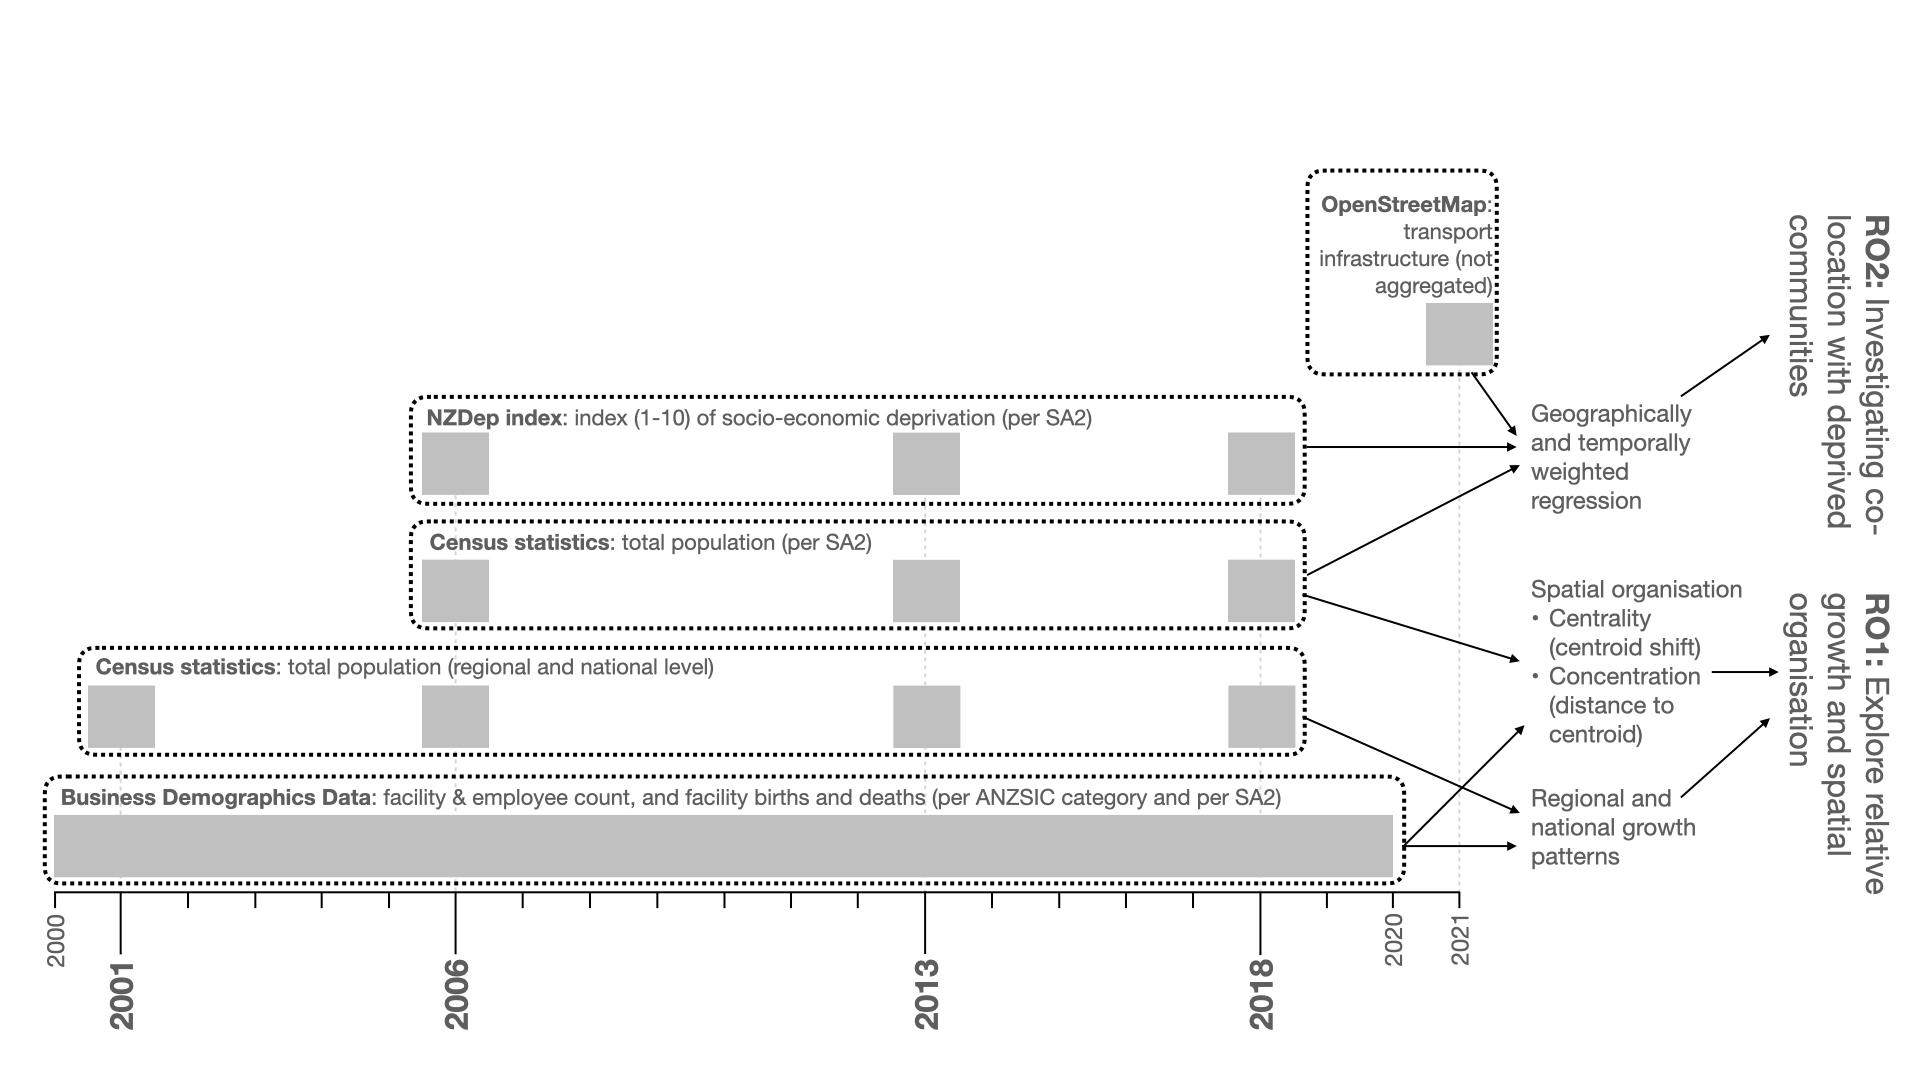
\includegraphics[width=0.9\linewidth]{methodology.jpeg}
    \caption{Graphic illustration of the research methodology.\nmt{remove birth and death stats - don't have for all industries}}
    \label{fig:method}
\end{figure}

%An important decision factor when choosing a location for a logistics facility is quick access to local, regional, and global transport networks \nmt{insert refs}. Highway networks are the most ubiquitous and truck transport the most flexible, therefore proximity to a highway network --- which can serve as an artery into local markets, connect regionally, or offer a direct route to a sea port or airport --- is an influential pull factor \nmt{insert refs}. Some studies have also found proximity to airports, railway terminals and seaports to be significantly influential \nmt{refs}. 

%In this study we've extracted the distance to the nearest airport, sea port, and railway terminal from the centroid of each \ac{SA2}. In terms of the highway network, we've opted to use the density of the highway network instead of the distance to the nearest highway on-ramp \nmt{insert ref that talks about why this is better}. We also decided to calculate the highway density for a larger geographic area than the \acp{SA2}, namely the \emph{urban} and \emph{rural} demarcations. The \acp{SA2} are small, geographically, in and around urban areas. Using such small areas to calculate highway densities would create distortions that imply that a logistics facility only considers the highway network immediately surrounding its facility and not the network in the rest of the urban area. 




%\subsection{Data sources and data sets}
%There are four sources of data for this study, illustrated in Figure~\ref{fig:DataSources}. Firstly, data regarding business facilities and employee counts --- differentiated by the \ac{ANZSIC} codes --- are from the annual Business Demography snapshot taken each February by \ac{StatsNZ}. Secondly, the \ac{NZDep} index data, which are calculated from the census statistics, are publicly available from the Health Inequalities Research Programme at the University of Otago \nmt{insert ref}. Thirdly, national census statistics are published by \ac{StatsNZ}. Finally, transport infrastructure data are drawn from \ac{OSM}.


%\subsubsection{Business demographics data}
%The business demographics data have been published annually by \ac{StatsNZ} since 2000. For confidentiality purposes, the published data is aggregated geographically on the \ac{SA2} level and functionally according to \ac{ANZSIC} codes. From this dataset, we've extracted the number of business facilities, employment per facility, and the number of ``births" and ``deaths" of business facilities for each year from 2000 to 2020.

%To serve the purposes of census data collection, \acp{SA2} are defined based on population counts and thus vary greatly in terms of area. As an illustration, Figure~\ref{fig:SA2} compares the size of \ac{SA2} in the city of Christchurch compared to the size of \acp{SA2} in the rest of the region. 


%Which \ac{ANZSIC} codes should be considered ``logistics facilities" is not immediately obvious. Consider the supply chain of flour for household use. Wheat is moved from farms to mills where it is transformed into flour and packaged for sale in grocery stores. Mills are the ``manufacturing facilities" in this supply chain. From the mill, pallets of packaged flour travel to a warehouse or distribution centre that is positioned closer to the consumer market. From there, flour can be transported to wholesale or retail outlets (or first to a wholesale and then to a retail outlet) where final consumers purchase the product. In this case the farm, the mill, the warehouse and/or distribution centre, the wholesale outlet, the retail outlet and any transport terminals involved are all logistics facilities.


%\subsubsection{Census statistics and the New Zealand Deprivation}

%To study the spatial organisation of urban logistics relative to how the population has moved and relative to community demographics, we draw from the national census statistics and the \ac{NZDep} index. The census was only conducted periodically in the past two decades (2001, 2006, 2013, and 2018) and not annually as in the case of the business demographics data. From the census data, we use the total population per \ac{SA2} to explore whether and how populations in the urban areas have grown(contracted) and sprawled(concentrated). However, the 2001 census data are reported on area unit level and not \ac{SA2} level and the reporting categories for many variables are different to the census categories for 2006, 2013, and 2018. Without a clear way of reconciling the data, the 2001 census statistics were omitted. 

%Studies that have investigated the relationship between urban logistics and low-income communities typically use a household income threshold to differentiate poorer communities form the rest. In this study, however, we do not only focus on income level, but wish to consider a broader definition of deprivation, therefore we use the \ac{NZDep} index instead of income variables. 

%The \ac{NZDep} index is a census-based, small-area index of relative socio-economic deprivation. The scale ranges from 1 to 10 with 10 indicating the highest level of deprivation. This index is frequently used in health and education related policy decisions in Aotearoa New Zealand. The interested reader is referred to \nmt{xx} and \nmt{xx} to read more about the theoretical and methodological underpinnings of the index. because it is census-based, updates have been published in 2001, 2006, 2013, and 2018. The \ac{NZDep} Index data could be aggregated to \ac{SA2} level for each of these four updates and so the 2001 data did not have to be excluded. In this study we rely exclusively on the \ac{NZDep} index to investigate the co-location of deprived communities and logistics facilities.


%The \ac{NZDep} index includes a broad range of deprivation dimensions and quantifies each with one or more variables from the census. The weighting of each dimension is statistically determined. Table~\ref{tab:NZDep2018} shows the variables included in the calculation of the 2018 index. Over time, the list of variables and their weightings have changed to stay abreast of societal developments. For example, not having access to internet at home is regarded an indicator of deprivation in 2018 whereas this was not the case decades earlier when internet at home was a luxury, not a basic necessity. The lists of variables used in 2001, 2006, and 2013 are shown in \ref{app:NZDep}. 

%To calculate the index on a scale from 1 to 10, the distribution of principal component scores derived from the variables is divided into tenths. The higher the index, the higher the deprivation. For example, an index of 10 for an area indicates that the area is in the most deprived 10 percent of small areas in New Zealand \nmt{ref the 2018 report}. 


%\begin{table}[h!]
 %   \centering
 %   \caption{The \ac{NZDep} deprivation dimensions and their concomitant variables for 2018 (ordered according to decreasing weight in the index). \nmt{ref}}
 %   \label{tab:NZDep2018}
%    \begin{tabular}{L{0.2\linewidth} L{0.7\linewidth} }
 %     \toprule
 %     Dimension of deprivation   & Description of variable \\
 %     \midrule
 %     Communication & People with no access to the Internet at home\\
 %     Income & People aged 18--64 receiving a means tested benefit\\
 %     Income & People living in equivalised households with income below an income threshold\\
 %     Employment & People aged 18-64 unemployed\\
 %     Qualifications & People aged 18-64 without any qualifications\\
 %     Owned home & People not living in own home\\
 %     Support & People aged $<$ 65 living in a single parent family\\
 %     Living space & People living in equivalised households below a bedroom occupancy threshold\\
%      Living condition & People living in dwellings that are always damp and/or always have mould greater than A4 size\\
 %     \bottomrule
%    \end{tabular}
%\end{table}



%\subsection{Census statistics}
%The census statistics used in this study relate to total population, ethnicity, employment, personal income, and household income \rs{At this stage, only total population is used as an independent variable in the correlation analysis, but I'm curious about your thoughts of unpacking things like education and ethinicity in the last sections of the paper.}. This data is publicly available and was downloaded from the \ac{StatsNZ} website \nmt{url}. These publicly available datasets are aggregated geographically and functionally (by \ac{ANZSIC} code). The data for 2006, 2013, and 2018 was available on the \ac{SA2} level. Unfortunately, the data for the 2001 census was not reported according to \ac{SA2} level but on area unit level. In addition, the reporting categories for personal income and workforce statistics, among others, were also different. Because we did not know how to map the area units to \acp{SA2} or how to reconcile the 2001 categories with the categories used since 2006, we decided to omit 2001 from the analysis and use only data from 2006, 2013, and 2018. 
%Because the census variable ``total population" is included as an independent \nmt{control?} variable in the correlation analyses, this decision to omit 


\section{Findings}
\label{sec:Findings}


\begin{figure}[h!]
    \centering
    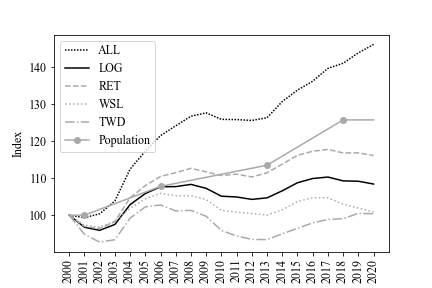
\includegraphics[width=0.9\linewidth]{IndexedGrowth.png}
    \caption{ccc}
    \label{fig:growth}
\end{figure}


\nmt{NADIA CONTINUE HERE}
\subsection{Exploring relative spatial organisation}
In studies of logistics sprawl, what constitutes ``logistics facilities" is interpreted differently, depending on the data sources. Most commonly, warehouses and distribution centres are considered logistics facilities. Some studies include transport terminals --- in other words, the facilities required to store and move goods along their journey from supplier to consumer. However, these two groups of facilities hardly address the overall scope of logistics. 

In this study of the spatial organisation of urban logistics, we include all facilities in the supply chain downstream of manufacturing. Manufacturing facilities and the sources of raw materials (farms, mines etc.) are excluded for two reasons. Firstly, the locations of farms and mines are mostly set and not affected by urban development. Secondly, there is less of an incentive for manufacturing facilities to be ``amidst the population". Distance to supplier is often more important than distance to consumer. We align the \ac{ANZSIC} categories to four categories of logistics facilities in this study as shown in Table~\ref{tab:Codes}. The fifth category in this study, ALL, includes all business facilities across all sectors of the economy and is used to compare trends between urban logistics facilities and business in general. 

\begin{table}[!h]
\caption{Alignment of study categories and ANZSIC codes}\label{tab:Codes}
\begin{tabular}{L{0.3\linewidth} c L{0.4\linewidth}}
\toprule
Study category & Study acronym & ANZSIC category\\
\midrule
Retail trade & RET & G (Retail trade)\\
\\
Wholesale trade & WSL & F (Wholesale trade)\\
\\
Transport terminals, warehousing \& distribution & TWD & I461 (road freight transport), I471 (rail freight transport), I481 (water freight transport), I51 (postal and courier pick-up), and I53 (warehousing and storage)\\ \\
All logistics facilities & LOG & All categories included for RET, WSL and TWD\\ \\
All business facilities & ALL & All ANZSIC categories are included\\
\bottomrule
\end{tabular}
\end{table}


\section{Discussion and conclusion}
\label{sec:DiscConc}

\nmt{Remember to highlight methodological novelties}

\section{Growth and densities over two decades}

Growth in national number of facilities (all industries) over 20 years has been 46\%. At the same time, the number of distribution facilities only grew by 1.5\% while the number of selling facilities grew by 10\%. This is interesting. How has the population grown between 2001 and 2018. In 2000, for every distribution facility there were 5.2 sell facilities and 35.3 other types of facilities (all - distrib - sell). In 2020, the ratio between distribution and sellside facilities did not change drastically (1:5.7), but for every distribution facility there are now 53.9 other types of facilities. \nmt{What is the significance of that?} 

The regions of Auckland, Canterbury, Waikato, and Wellington had the most logistics facilities (in absolute terms) in 2020. This is unsurprising. 

%
\begin{figure}[h!]
\subfloat[All industries\label{fig:PieTotInd}]{
	\begin{minipage}[t]{0.30\linewidth}
	\centering
	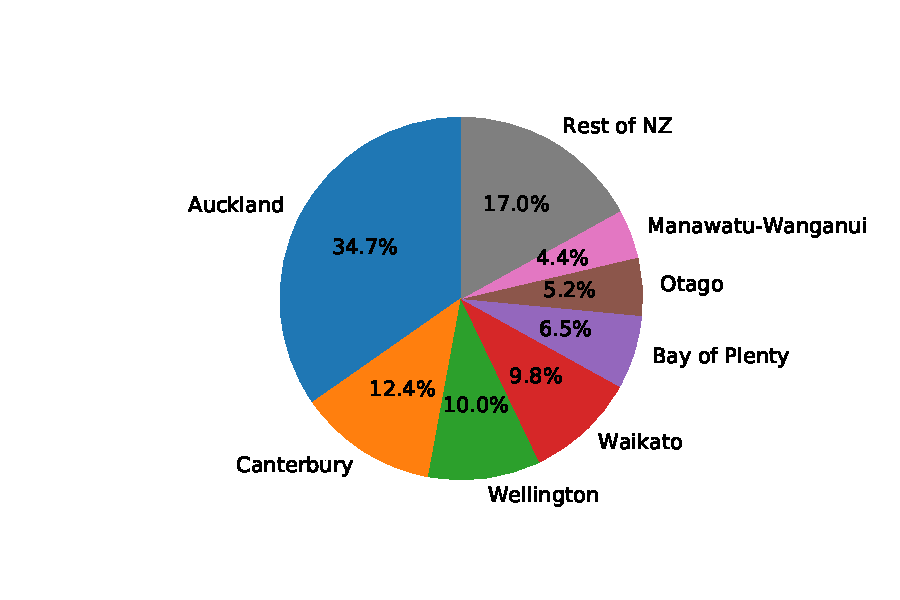
\includegraphics[width=1\linewidth]{PieTot_2020} \medskip \\
	\end{minipage}
}\hfill
\subfloat[Transport \& storage\label{fig:PieDistrib}]{
	\begin{minipage}[t]{0.30\linewidth}
	\centering
	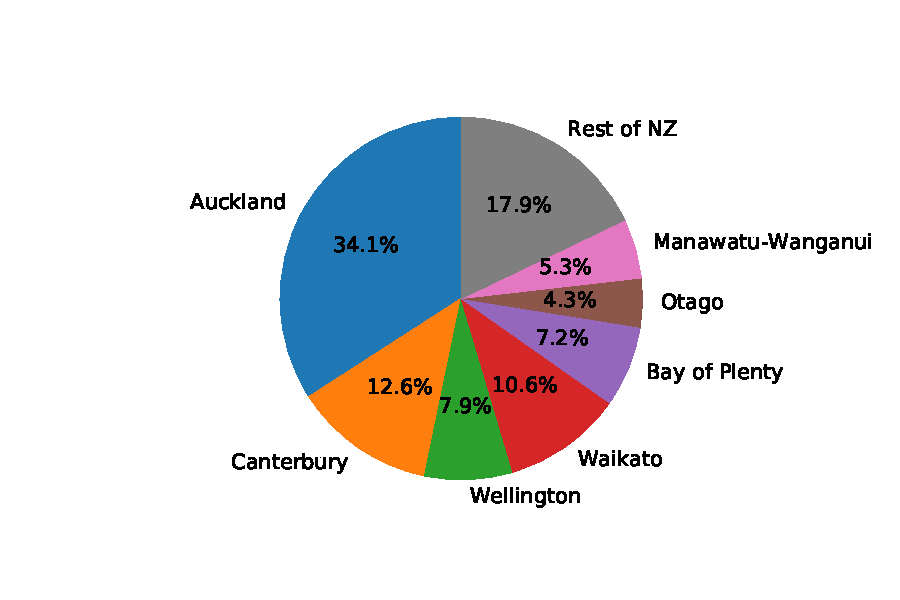
\includegraphics[width=1\linewidth]{PieDistr_2020} \medskip \\
	\end{minipage}
}\hfill
\subfloat[Wholesale \& retail\label{fig:PieSell}]{
	\begin{minipage}[t]{0.30\linewidth}
	\centering
	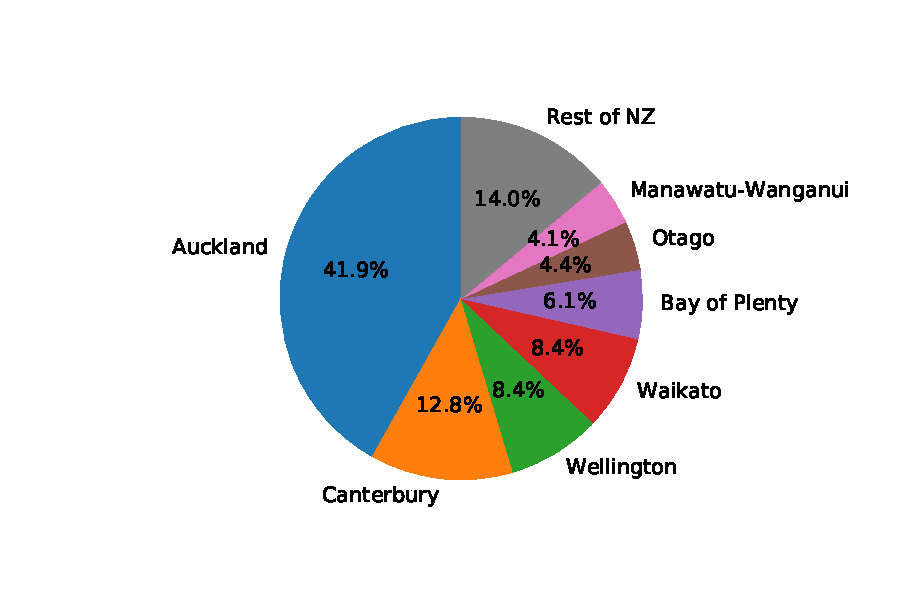
\includegraphics[width=1\linewidth]{PieSell_2020} \medskip \\
	\end{minipage}}
\caption{Percentage of national facilities in each region (2020)}\label{fig:PercOfFac}
\end{figure}
%

The contributions of the different regions have remained relatively stable in each area for each type of facility. 

\begin{table}[!h]
\caption{Some cap}\label{tab:regionCompLongit}
\resizebox{\textwidth}{!}{%
	\begin{tabular}{l c r r r r r c r r r r r c r r r r r c r c r}
	\toprule
	Region&&\multicolumn{5}{c}{All industries}&&\multicolumn{5}{c}{Distribution}&&\multicolumn{5}{c}{Selling}&&Pop&&GDP\\
	&&\rotatebox{90}{2000}&\rotatebox{90}{2005}&\rotatebox{90}{2010}&\rotatebox{90}{2015}&\rotatebox{90}{2020}&&\rotatebox{90}{2000}&\rotatebox{90}{2005}&\rotatebox{90}{2010}&\rotatebox{90}{2015}&\rotatebox{90}{2020}&&\rotatebox{90}{2000}&\rotatebox{90}{2005}&\rotatebox{90}{2010}&\rotatebox{90}{2015}&\rotatebox{90}{2020}&&2018&&2019\\
	\midrule
	Auckland&&30.3&31.4&31.4&33.2&34.7&&34.0&32.9&31.9&33.2&34.1&&37.3&38.4&39.0&41.6&41.9&&33.4&&37.6\\
	Canterbury&&12.3&12.5&12.6&12.9&12.4&&11.9&12.3&12.6&12.9&12.6&&13.3&13.5&13.5&12.9&12.8&&12.8&&12.4\\
	Waikato&&10.6&10.3&10.1&9.9&9.8&&10.1&10.5&10.5&10.1&10.6&&8.4&8.4&8.3&8.2&8.4&&9.7&&8.5\\
	Wellington&&10.5&10.1&10.2&10.0&10.0&&9.6&8.7&8.6&8.4&7.9&&10.4&9.6&9.3&8.8&8.4&&10.8&&12.9\\
	Bay of Plenty&&6.5&6.7&6.6&6.4&6.5&&7.0&6.9&7.0&6.8&7.2&&6.1&6.1&6.2&5.9&6.1&&6.6&&5.7\\
	Manawatu-Wanganui&&5.7&5.3&5.1&4.7&4.4&&6.0&6.1&5.9&5.5&5.3&&5.1&4.7&4.5&4.2&4.1&&5.1&&3.8\\
	Otago&&4.6&4.9&5.1&5.2&5.2&&4.1&4.6&4.6&4.4&4.3&&4.3&4.3&4.4&4.3&4.4&&4.8&&4.5\\
	Rest of NZ&&19.5&18.9&18.7&17.8&17.0&&17.3&18.0&18.9&18.6&17.9&&15.2&14.8&14.8&14.0&14.0&&16.8&&14.7\\
	\bottomrule
	\end{tabular}}

\end{table}



\nmt{Next look at growth rates and birth/death rates of facilities (first need to create C stats)}

\section{Regions in spatial detail}
Only Auckland, Canterbury, Wellington, Waikato

\addcontentsline{toc}{section}{References}
\section*{References}
\bibliography{logisticSprawl_NZ.bib}


\end{document}
